\documentclass[a4paper,12pt,onecolumn]{article}

\usepackage[T1]{fontenc}
\usepackage[utf8]{inputenc}
\usepackage[english]{babel}
\usepackage{amssymb,amsmath,amsthm,array,epsfig,lmodern,pstricks,subfig,hyperref
,verbatim,textcomp}
\newtheorem{thm}{Theorem}
\newtheorem{lem}[thm]{Lemma}
\newtheorem{rem}[thm]{Remark}

\newenvironment{keywords}{{\upshape\bfseries Key words. }\ignorespaces}{}

\newcommand{\R}{{\mathbb R}}
\newcommand{\vol}{\mathcal{L}^d}
\newcommand{\dH}[1]{\;{\rm d}{\cal H}^{#1}} % Hausdorff measure
\newcommand{\dL}[1]{\;{\rm d}{\cal L}^{#1}} % Lebesgue measure
\newcommand{\bigchi}{\ensuremath{\mathrm{\mathcal{X}}}}
\newcommand{\charfcn}[1]{\bigchi_{#1}} % characteristic function
\newcommand{\Vh}{\underline{V}(\Gamma^m)}
\newcommand{\Wh}{W(\Gamma^m)}
\newcommand{\Vht}{\underline{V}(\Gamma^h(t))}
\newcommand{\Wht}{W(\Gamma^h(t))}
\newcommand{\uspace}{\mathbb{U}}
\newcommand{\pspace}{\mathbb{P}}
\newcommand{\kspace}{\mathbb{K}}
\newcommand{\xspace}{\mathbb{X}}
\newcommand{\sigmaO}{o}
\newcommand{\nabs}{\nabla_{\!s}}
\newcommand{\id}{\rm id}
\newcommand{\ddt}{\frac{\rm d}{{\rm d}t}}
\newcommand{\NbulkT}{\vec{N}_{\Gamma,\Omega}^T}
\newcommand{\Nbulk}{\vec{N}_{\Gamma,\Omega}}
\newcommand{\errorXx}{\|\Gamma^h - \Gamma\|_{L^\infty}}
\newcommand{\LerrorUu}[1]{\|\vec U - I^h_{#1}\,\vec u\|_{L^2}}
\newcommand{\HerrorUu}[1]{\|\vec U - I^h_{#1}\,\vec u\|_{H^1}}
\newcommand{\LerrorPp}{\|P - p\|_{L^2}}
\newcommand{\unitn}{\vec{\rm n}}
\newcommand{\mat}[1]{\underline{\underline{#1}}\rule{0pt}{0pt}}
\newcommand{\strikec}{\mbox{$c\!\!\!\!\:/$}}
\newcommand{\Mloss}{\mathcal{L}_{\rm loss}}
\newcommand{\ek}{e}

\renewcommand{\theequation}{\arabic{section}.\arabic{equation}}

\textwidth 425pt

\title{Fitted Finite Element Discretization of \\ Two-Phase Navier--Stokes
Flow using an ALE formulation}
\author{Marco Agnese and Robert N\"urnberg%
\thanks{email: \texttt{\{m.agnese13,robert.nurnberg\}@imperial.ac.uk}}\\
\small
Department of Mathematics, Imperial College, London, SW7 2AZ, U.K.}
\date{}

\begin{document}

\captionsetup[subfigure]{labelformat=empty} % remove label subplot

\maketitle

\begin{abstract}
We propose a novel fitted finite element method for two-phase Navier-Stokes
flow problems that uses piecewise linear finite elements to approximate the
moving interface. We present several numerical experiments for our numerical
method, which demonstrate the accuracy and robustness of the proposed algorithm.
\end{abstract}

\begin{keywords}
incompressible two-phase flow, Navier--Stokes equations,
free boundary problem, surface tension, finite elements, front tracking, ALE
\end{keywords}

\section{Mathematical model} \label{sec:model}

\subsection{Governing equations}\label{sec:equations}
TODO: add free slip condition

In this paper we consider two-phase Navier--Stokes flow in a given domain
$\Omega\subset\mathbb{R}^d$, where $d=2$ or $d=3$. The domain $\Omega$ contains
two different immiscible, incompressible, fluids (liquid-liquid or
liquid-gas) which for all $t\in[0,T]$ occupy time dependent regions
$\Omega_+(t)$ and $\Omega_-(t):=\Omega\setminus\overline{\Omega}_+(t)$ and
which are separated by an interface
$(\Gamma(t))_{t\in[0,T]}$, $\Gamma(t)\subset\Omega$.
See Figure~\ref{fig:sketch} for an illustration.
\begin{figure}
\begin{center}
\unitlength15mm
\psset{unit=\unitlength,linewidth=1pt}
\begin{picture}(4,4)(0,0)
\psline(0,0)(4,0)(4,4)(0,4)(0,0)
\psellipse(2,2)(1,1)
\psline{->}(3,2)(3.5,2)
\put(3.25,1.75){$\vec\nu$}
\put(1.75,0.75){{$\Gamma(t)$}}
\put(1.75,2){{$\Omega_-(t)$}}
\put(0.5,3.25){{$\Omega_+(t)$}}
\end{picture}
\end{center}
\caption{The domain $\Omega$ in the case $d=2$.}
\label{fig:sketch}
\end{figure}
For later use, we assume that $(\Gamma(t))_{t\in [0,T]}$ is a sufficiently
smooth evolving hypersurface without boundary. Let
$\vec x(\cdot,t):\Upsilon\to\R^d$ be an homeomorphic map which at each time
$t\in [0,T]$ associates a point $\vec q$ of a reference manifold
$\Upsilon\subset \R^d$ to a point $\vec z\in \Omega$:
\begin{equation}\label{eq:x}
\vec x(\cdot,t):\Upsilon\to\Omega, \qquad \vec z=\vec x(t,\vec q).
\end{equation}
Therefore, given a suitable $\Upsilon_{\Gamma}$, we can parametrize the
evolving interface as $\Gamma(t) = \vec x(\Upsilon_{\Gamma},t)$ with velocity
\begin{equation} \label{eq:V}
\vec{\mathcal{V}}(\vec z, t) := \vec x_t(\vec q, t) \qquad
\forall\ \vec z = \vec x(\vec q,t) \in \Gamma(t)
\end{equation}
where $\vec{\mathcal{V}} \,.\,\vec{\nu}$ is the normal velocity of the evolving
hypersurface $\Gamma(t)$ and $\vec\nu(t)$ is the unit normal on $\Gamma(t)$
pointing into $\Omega_+(t)$.

Denoting the velocity and pressure by $\vec u$ and $p$, respectively, we
introduce the stress tensor
\begin{equation} \label{eq:stress_tensor}
\mat\sigma = \mu \,(\nabla\,\vec u + (\nabla\,\vec u)^T) - p\,\mat\id
= 2\,\mu\, \mat D(\vec u)-p\,\mat\id\,,
\end{equation}
where $\mu(t) = \mu_+\,\charfcn{\Omega_+(t)} + \mu_-\,\charfcn{\Omega_-(t)}$,
with $\mu_\pm \in \R_{>0}$, denotes the dynamic viscosities in the two phases,
$\mat\id \in \R^{d \times d}$ is the identity matrix and
$\mat D(\vec u):=\frac{1}{2}\, (\nabla\vec u+(\nabla\vec u)^T)$
is the rate-of-deformation tensor. Finally let
$\rho(t) = \rho_+\,\charfcn{\Omega_+(t)} + \rho_-\,\charfcn{\Omega_-(t)}$,
with $\rho_\pm \in \R_{>0}$, be the fluid density.

In this paper we consider a two-phase Navier--Stokes problem, and so the
equations governing the fluid are
\begin{subequations}
\begin{alignat}{2}
\rho\,(\vec u_t +\vec u \,.\, \nabla \vec u)- \nabla\,.\,\mat\sigma
& = \vec f \qquad &&\mbox{in } \Omega_\pm(t)\,,
\label{eq:ns_momentum} \\
\nabla\,.\,\vec u & = 0 \qquad &&\mbox{in } \Omega_\pm(t)\,,
\label{eq:ns_mass}
\end{alignat}
\end{subequations}
where $\vec f$ is a possible forcing term.

On the free surface $\Gamma(t)$, the following conditions need to hold:
\begin{subequations}
\begin{alignat}{2}
[\vec u]_-^+ & = \vec 0 \qquad &&\mbox{on } \Gamma(t)\,,
\label{eq:interface_jump_velocity} \\
[\mat\sigma\,\vec \nu]_-^+ & = -\gamma\,\varkappa\,\vec\nu \qquad
&&\mbox{on } \Gamma(t)\,, \label{eq:interface_jump_stress} \\
\vec{\mathcal{V}}\,.\,\vec\nu &= \vec u\,.\,\vec \nu \qquad
&&\mbox{on } \Gamma(t)\,, \label{eq:interface_velocity}
\end{alignat}
\end{subequations}
where $\gamma>0$ is the surface tension coefficient and $\varkappa$ denotes the
mean curvature of $\Gamma(t)$, i.e.\ the sum of the principal curvatures of
$\Gamma(t)$, where we have adopted the sign convention that $\varkappa$ is
negative where $\Omega_-(t)$ is locally convex. In particular,
see e.g.\ \cite{DeckelnickDE05}, it holds that
\begin{equation} \label{eq:LBop}
\Delta_s\, \vec \id = \varkappa\, \vec\nu \qquad \mbox{on $\Gamma(t)$}\,,
\end{equation}
where $\Delta_s = \nabs\,.\,\nabs$ is the Laplace--Beltrami operator on
$\Gamma(t)$ with $\nabs\,.\,$ and $\nabs$ denoting surface divergence and
surface gradient on $\Gamma(t)$, respectively. Moreover, as usual,
$[\vec u]_-^+ := \vec u_+ - \vec u_-$ and
$[\mat\sigma\,\vec\nu]_-^+ := \mat\sigma_+\,\vec\nu - \mat\sigma_-\,\vec\nu$
denote the jumps in velocity and normal stress across the interface
$\Gamma(t)$. Here and throughout, we employ the shorthand notation
$\vec g_\pm := \vec g\!\mid_{\Omega_\pm(t)}$ for a function
$\vec g : \Omega \times [0,T] \to \R^d$; and similarly for scalar and
matrix-valued functions. To close the system we prescribe the initial data
$\Gamma(0) = \Gamma_0$, the initial velocity $\vec u(0) = \vec u_0$ and the
boundary condition $\vec u = \vec 0$ on $\partial \Omega$.

\subsection{Arbitrary Lagrangian Eulerian (ALE) formulation}\label{sec:ale}
TODO: specify that we have only one map $\vec x$ defined over
$\Upsilon_{\Omega_-}\cup\Upsilon_{\Omega_+}\cup\Upsilon_{\Gamma}$. Unify
definition domain velocities like $\mathcal{V}_\Gamma$ and
$\mathcal{V}_{\Omega_\pm}$ (also at discrete level).

The system of governing equations
(\ref{eq:ns_momentum},\ref{eq:ns_mass},\ref{eq:interface_jump_velocity},
\ref{eq:interface_jump_stress},\ref{eq:interface_velocity}) is expressed in
term of Eulerian coordinates $\vec z$. It is possible to rewrite the velocity
time derivative $\vec u_t$ respect to the so called ALE coordinate $\vec q$.

Analogously of what done in Section~\ref{sec:equations} to parametrize the
interface $\Gamma(t)$, we can define the fixed reference manifolds
$\Upsilon_{\Omega_-}$ and $\Upsilon_{\Omega_+}$ and use the map
(\ref{eq:x}) to parametrize $\Omega_\pm(t)$ as
$\Omega_-(t)=\vec x(\Upsilon_{\Omega_-},t)$ and $\Omega_+(t)=\vec
x(\Upsilon_{\Omega_+},t)$.

Now, let $h:\Omega_{\pm}(t)\times [0,T]\to \mathbb{R}$ be a function defined on
the Eulerian frame, the corresponding function on the ALE frame $\hat h$ is
defined as
\begin{equation}\label{eq:h}
\hat h:\Upsilon_{\Omega_\pm}\times [0,T]\to \mathbb{R},\qquad
\hat h(\vec q,t)=h(\vec{x}(\vec q,t),t).
\end{equation}
In order to compute the time derivative of (\ref{eq:h}) with respect to the ALE
frame, using the chain rule, we have
\begin{equation}
\frac{\partial\hat h(\vec q,t)}{\partial t}=\frac{\partial h(\vec x(\vec
q,t),t)}{\partial t}=\frac{\partial h(\vec z,t)}{\partial t}+\vec x_t(\vec q,t)
\cdot \nabla h(\vec z,t),
\end{equation}
therefore it holds that
\begin{equation}
\frac{\partial h(\vec z,t)}{\partial t} =
\frac{\partial\hat h(\vec q,t)}{\partial t}-
\vec x_t(\vec q,t) \cdot \nabla h(\vec z,t).
\end{equation}
Finally, introducing the domain velocity
\begin{equation} \label{eq:W}
\vec{\mathcal{W}}(\vec z, t) := \vec x_t(\vec q, t) \qquad
\forall\ \vec z = \vec x(\vec q,t) \in \Omega_\pm(t)
\end{equation}
and the time derivative in the ALE frame
\begin{equation} \label{eq:ale_derivative}
\left.\frac{\partial h(\vec z,t)}{\partial t}\right|_{\Upsilon_{\Omega_\pm}}:=
\frac{\partial\hat h(\vec q,t)}{\partial t} \qquad
\forall\ \vec z = \vec x(\vec q,t) \in \Omega_\pm(t)
\end{equation}
we obtain
\begin{equation}\label{eq:ale_dt}
h_t =\left.h_t\right|_{\Upsilon_{\Omega_\pm}} -\vec{\mathcal{W}} \cdot \nabla h.
\end{equation}

Using (\ref{eq:ale_dt}) in (\ref{eq:ns_momentum}), we can now write the full
system of governing equations in an Arbitrary Lagrangian Eulerian frame as:
\begin{subequations}
\begin{alignat}{2}
\rho\,(\left.\vec{u}_t\right|_{\Upsilon_{\Omega_\pm}}
+(\vec u - \vec{\mathcal{W}})\,.\, \nabla \vec u)\,
-2 \mu\,\nabla\,.\, \mat D(\vec u)+ \nabla\,p & = \vec f
\quad &&\mbox{in } \Omega_\pm(t)\,, \label{eq:full_momentum} \\
\nabla\,.\,\vec u & = 0 \quad &&\mbox{in } \Omega_\pm(t)\,,
\label{eq:full_mass} \\
\vec u & = \vec 0 \qquad &&\mbox{on } \partial\Omega\,,
\label{eq:full_initial_velocity} \\
[\vec u]_-^+ & = \vec 0 \quad &&\mbox{on } \Gamma(t)\,,
\label{eq:full_jump_velocity} \\
[2\mu \,\mat D(\vec u)\,.\,\vec\nu - p\,\vec \nu]_-^+
& = -\gamma\,\varkappa\,\vec\nu
\quad &&\mbox{on } \Gamma(t)\,, \label{eq:full_jump_stress} \\
(\vec{\mathcal{V}}-\vec u)\,.\,\vec{\nu} & = 0
\quad &&\mbox{on } \Gamma(t)\,,\label{eq:full_velocity}  \\
\Gamma(0) & = \Gamma_0 \,.\label{eq:full_initial_interface}
\end{alignat}
\end{subequations}
We can notice that, with respect to the original formulation, there is a
convective-type term due to the domain movement and the time derivative is
computed in the fixed reference frame $\Upsilon_{\Omega_\pm}$. Obviously, if
the domain is fixed, this additional convective term is zero and the time
derivative in the ALE frame coincide with the usual time derivative in the
Eulerian frame.

\subsection{Weak formulation}\label{sec:weak}
TODO: add definition space of ALE counterpart

In order to obtain a weak formulation, we define the function spaces
\begin{align*}
\uspace &:= [H^1_0(\Omega)]^d\,,\qquad \pspace := L^2(\Omega) \qquad
\mbox{and}\qquad
\widehat\pspace := \{\eta\in\pspace : \int_\Omega\eta\dL{d}=0 \}\,,
\end{align*}
and let $(\cdot,\cdot)$ and $\langle \cdot, \cdot \rangle_{\Gamma(t)}$ denote
the $L^2$--inner products on $\Omega$ and $\Gamma(t)$, respectively. In
addition, we let $\mathcal{L}^d$ and $\mathcal{H}^{d-1}$ denote the Lebesgue
measure in $\R^d$ and the $(d-1)$-dimensional Hausdorff measure, respectively.

Multiplying (\ref{eq:LBop}) with a test function, and performing integration by
parts, yields
\begin{equation*}
\left\langle \varkappa\,\vec\nu, \vec\eta \right\rangle_{\Gamma(t)}
+ \left\langle \nabs\,\vec \id, \nabs\,\vec \eta \right\rangle_{\Gamma(t)}
= 0  \quad \forall\ \vec\eta \in [H^1(\Gamma(t))]^d\,.
\end{equation*}
Moreover, on noting (\ref{eq:stress_tensor}) and
(\ref{eq:interface_jump_stress}), we have that
\begin{align*}
\int_{\Omega_+(t)\cup\Omega_-(t)} (\nabla\,.\,\mat\sigma)\,.\, \vec \xi \dL{d}
& = - \left(\mat\sigma, \nabla\,\vec \xi\right)
- \left\langle [\mat\sigma\,\vec\nu]_-^+ , \vec \xi
  \right\rangle_{\Gamma(t)} \nonumber \\
& = \left( p , \nabla\,.\,\vec \xi\right)
-2 \left(\mu\,\mat D(\vec u) , \mat D(\vec \xi) \right)
+ \gamma \left\langle \varkappa\,\vec \nu , \vec \xi  \right\rangle_{\Gamma(t)}
\end{align*}
for all $\vec \xi \in [H^1_0(\Omega)]^d$.

Hence a possible weak formulation of
(\ref{eq:full_momentum}--g) is given as follows. Given $\Gamma(0) = \Gamma_0$,
for almost all $t\in(0,T)$ find $\Gamma(t)$ and ${(\vec u, p, \varkappa)}$ ${\in
\uspace \times \widehat\pspace \times H^1(\Gamma(t))}$ such that
\begin{subequations}
\begin{align}
& (\rho\,\left.\vec{u}_t\right|_{\Upsilon_{\Omega_\pm}}, \vec \xi)
+ (\rho\,(\vec u - \vec{\mathcal{W}})\,.\,\nabla\,
\vec u\,,\,\vec \xi) +2\left(\mu\,\mat D(\vec u), \mat D(
\vec \xi)\right) \nonumber \\
& - \left(p, \nabla\,.\,\vec \xi\right)
- \gamma\,\left\langle \varkappa\,\vec\nu, \vec\xi\right\rangle_{\Gamma(t)}
= \left(\vec f, \vec \xi\right)\quad \forall\ \vec\xi \in \uspace \,,
\label{eq:weaka}\\
& \left(\nabla\,.\,\vec u, \varphi\right) = 0
\quad \forall\ \varphi \in \widehat\pspace\,, \label{eq:weakb} \\
&  \left\langle \vec{\mathcal{V}}
- \vec u, \chi\,\vec\nu \right\rangle_{\Gamma(t)} = 0
\quad \forall\ \chi \in H^1(\Gamma(t))\,, \label{eq:weakc} \\
& \left\langle \varkappa\,\vec\nu, \vec\eta \right\rangle_{\Gamma(t)}
+ \left\langle \nabs\,\vec \id, \nabs\,\vec \eta \right\rangle_{\Gamma(t)}
= 0  \quad \forall\ \vec\eta \in [H^1(\Gamma(t))]^d \label{eq:weakd}
\end{align}
\end{subequations}
holds for almost all times $t \in (0,T]$. Here we have observed that if
$p \in \pspace$ is part of a solution to (\ref{eq:full_momentum}--g), then so is
$p + c$ for an arbitrary $c\in \R$.

\subsection{Alternative antisymmetric weak formulation}

We note that in Section~\ref{sec:weak} we are using a different, and more
standard, weak formulation respect to paper \cite{fluidfbp}. There the authors
use \cite[eq. 3.7]{fluidfbp} in order to obtain a weak formulation for which it
is easy to derive an energy bound not only on the continuous level but also on
discrete level, as well as existence/uniqueness on discrete level. For
completeness we report the derivation of that antisymmetric weak formulation.

First, we observe that for arbitrary functions $\vec v$,
$\vec \omega$, $\vec \xi \in H^1(\Omega,\R^d)$ it holds that
\begin{align} \label{eq:tripleterm}
[(\vec v\,.\,\nabla)\,\vec \omega]\,.\,\vec \xi
&= (\vec v\,.\,\nabla)\,(\vec \omega\,.\,\vec \xi) -
[(\vec v\,.\,\nabla)\,\vec \xi]\,.\,\vec \omega \nonumber \\ &
= \tfrac{1}{2} \left[\,
[(\vec v\,.\,\nabla)\,\vec \omega]\,.\,\vec \xi - [(\vec v\,.\,\nabla)\,\vec
\xi] \,.\,\vec \omega\,\right] + \tfrac{1}{2}\,(\vec v\,.\,\nabla)\,
(\vec \omega\,.\,\vec \xi)\,.
\end{align}

Then we have for any $\vec v \in \uspace$ that
\begin{align} \label{eq:ibp0}
( \rho,(\vec v \,.\,\nabla)\,\phi) & = (\rho, \nabla\,.\,(\phi\,\vec v))
- (\rho\,(\nabla\,.\,\vec v), \phi) \nonumber \\ & =
- \left\langle [\rho]_-^+\,\vec v\,.\,\vec \nu,
  \phi \right\rangle_{\Gamma(t)}
- (\rho\,(\nabla\,.\,\vec v), \phi)
\end{align}
which holds for all $\phi\in W^{1,\frac{3}{2}}(\Omega)$, and it is
precisely this regularity that will be needed in order to derive
(\ref{eq:advect}) below.

Hence, it follows from (\ref{eq:full_momentum}),
(\ref{eq:tripleterm}) and (\ref{eq:ibp0}) that
\begin{align}\label{eq:fulladvect}
& ( \rho\,(\vec u \,.\,\nabla)\,\vec u, \vec \xi)
= \tfrac{1}{2} [ (\rho\,(\vec u\,.\,\nabla)\,\vec u, \vec \xi) -
(\rho\,(\vec u\,.\,\nabla)\,\vec \xi,\vec u) \nonumber \\
& -\langle [\rho]_-^+\vec u\,.\,\vec \nu, \vec u\,.\,\vec \xi
\rangle_{\Gamma(t)} -(\rho\,(\nabla\,.\,\vec u ),\vec u\,.\,\vec\xi) ] \qquad
\forall\ \vec \xi \in H^1(\Omega,{\mathbb R}^d)\,,
\end{align}
and from (\ref{eq:full_mass}) we obtain
\begin{align}\label{eq:advect}
& ( \rho\,(\vec u \,.\,\nabla)\,\vec u, \vec \xi)
= \tfrac{1}{2} [ (\rho\,(\vec u\,.\,\nabla)\,\vec u, \vec \xi) -
(\rho\,(\vec u\,.\,\nabla)\,\vec \xi,\vec u) \nonumber \\
& -\langle [\rho]_-^+\vec u\,.\,\vec \nu, \vec u\,.\,\vec \xi
\rangle_{\Gamma(t)}] \qquad \forall\ \vec \xi \in H^1(\Omega,{\mathbb R}^d)\,.
\end{align}

Next, on noting (\ref{eq:advect}) and using Reynolds transport theorem,
we have that
\begin{align}
\ddt(\rho \,\vec u, \vec \xi) & =
\ddt\left(\rho_+\,\int_{\Omega_+(t)} \vec u \,.\,\vec \xi \dL{d}
+ \rho_-\,\int_{\Omega_-(t)} \vec u\,.\,\vec \xi \dL{d}  \right) \nonumber \\
& =  (\rho\,\vec u_t, \vec \xi)
-\left\langle [\rho]_-^+\,\mathcal{V}, \vec u \,.\,\vec \xi
\right\rangle_{\Gamma(t)} \nonumber \\
&= (\rho\,\vec u_t, \vec \xi)- \left\langle [\rho]_-^+\,\vec u\,.\,\vec \nu,
\vec u \,.\,\vec \xi \right\rangle_{\Gamma(t)}
\qquad \forall \vec \xi \in H^1(\Omega, {\mathbb R}^d)\,.
\label{eq:rhot1}
\end{align}
Therefore, it follows from (\ref{eq:rhot1}) that
\begin{equation*}
(\rho\,\vec u_t, \vec \xi) =
\tfrac{1}{2} \left[
\ddt (\rho\,\vec u,\vec \xi) + (\rho\,\vec u_t, \vec \xi)
+ \left\langle [\rho]_-^+\,\vec u\,.\,\vec \nu,
\vec u \,.\,\vec \xi \right\rangle_{\Gamma(t)}
\right]
\qquad \forall\ \vec \xi \in H^1(\Omega, {\mathbb R}^d)\,,
\end{equation*}
which on combining with (\ref{eq:advect}) yields that
\begin{align} \label{eq:rhot3}
& (\rho\,[\vec u_t + (\vec u\,.\,\nabla)\,\vec u], \vec \xi) \nonumber \\
& = \tfrac{1}{2}\bigg[ \ddt (\rho\,\vec u, \vec \xi)
+ (\rho\,\vec u_t, \vec \xi) + (\rho, [(\vec u\,.\,\nabla)\,\vec u]\,.\,\vec \xi
- [(\vec u\,.\,\nabla)\,\vec \xi]\,.\,\vec u) \bigg].
\end{align}

Hence an alternative antisymmetric weak formulation of
(\ref{eq:full_momentum}--g) is given as follows. Given $\Gamma(0) = \Gamma_0$,
for almost all $t\in(0,T)$ find $\Gamma(t)$ and ${(\vec u, p, \varkappa)}$ ${\in
\uspace \times \widehat\pspace \times H^1(\Gamma(t))}$ such that
\begin{subequations}
\begin{align}
& \tfrac{1}{2}[ \ddt (\rho\,\vec u, \vec \xi) + (\rho\,\vec u_t, \vec \xi)
+ (\rho, [(\vec u\,.\,\nabla)\,\vec u]\,.\,\vec \xi
- [(\vec u\,.\,\nabla)\,\vec \xi]\,.\,\vec u) \nonumber \\
& +2\left(\mu\,\mat D(\vec u), \mat D(\vec \xi)\right)
- \left(p, \nabla\,.\,\vec \xi\right)
- \gamma\,\left\langle \varkappa\,\vec\nu, \vec\xi\right\rangle_{\Gamma(t)}
= \left(\vec f, \vec \xi\right)\quad \forall\ \vec\xi \in \uspace \,,
\label{eq:altweaka}\\
& \left(\nabla\,.\,\vec u, \varphi\right) = 0
\quad \forall\ \varphi \in \widehat\pspace\,, \label{eq:altweakb} \\
&  \left\langle \vec{\mathcal{V}}
- \vec u, \chi\,\vec\nu \right\rangle_{\Gamma(t)} = 0
\quad \forall\ \chi \in H^1(\Gamma(t))\,, \label{eq:altweakc} \\
& \left\langle \varkappa\,\vec\nu, \vec\eta \right\rangle_{\Gamma(t)}
+ \left\langle \nabs\,\vec \id, \nabs\,\vec \eta \right\rangle_{\Gamma(t)}
= 0  \quad \forall\ \vec\eta \in [H^1(\Gamma(t))]^d \label{eq:altweakd}
\end{align}
\end{subequations}
holds for almost all times $t \in (0,T]$.

\begin{rem} \label{rem:velocityhs}
With a view towards some numerical test cases
in Section~\ref{sec:numerical_results}, we also allow for non divergence-free
problem therefore (\ref{eq:advect}) is no longer valid and we need to use
(\ref{eq:fulladvect}) to derive the antisymmetric weak formulation.
Consequently the RHS of (\ref{eq:altweaka}) requires the additional term
\begin{equation} \label{eq:additionalvelocityrhs}
\tfrac{1}{2}(\rho\,(\nabla\,.\,\vec u ),\vec u\,.\,\vec\xi)\,.
\end{equation}
\end{rem}

\subsection{Finite element approximation}
TODO: formulate as iterative scheme, state stopping criteria

We consider the partitioning  $0= t_0 < t_1 < \ldots < t_{M-1} < t_M = T$ of
$[0,T]$ into possibly variable time steps
$\tau_m := t_{m+1}-t_m$, $m=0 ,\ldots, M-1$. Moreover, let
${\cal T}^m$, $\forall m\ge 0$, be a regular partitioning of the domain
$\Omega$ into disjoint open simplices
$\sigmaO^m_j$, $j = 1 ,\ldots, J^m_\Omega$. On ${\cal T}^m$ we define the
finite element spaces
\begin{equation*}
S^m_k := \{\chi \in C(\overline{\Omega}) : \chi\!\mid_{\sigmaO^m}
\in \mathcal{P}_k(\sigmaO^m) \ \forall\ \sigmaO^m \in {\cal T}^m\}
\subset H^1(\Omega),\quad k \in \mathbb{N}\,,
\end{equation*}
where $\mathcal{P}_k(\sigmaO^m)$ denotes the space of polynomials of degree $k$
on $\sigmaO^m$. Moreover, $S^m_0$ is the space of piecewise constant functions
on ${\cal T}^m$.

Let $\uspace^m\subset\uspace$ and $\pspace^m\subset\pspace$ be the finite
element spaces we use for the approximation of velocity and pressure,
and let $\widehat\pspace^m:= \pspace^m \cap \widehat\pspace$.
The spaces $(\uspace^m,\pspace^m)$ satisfy the LBB inf-sup condition if there
exists a constant $C_0 \in \R_{>0}$, independent of $\mathcal{T}^m$, such that
\begin{equation} \label{eq:LBB}
\inf_{\varphi \in \widehat\pspace^m} \sup_{\vec \xi \in \uspace^m}
\frac{( \varphi, \nabla \,.\,\vec \xi)} {\|\varphi\|_0\,\|\vec \xi\|_1}
\geq C_0 > 0\,,
\end{equation}
see \cite[p.~114]{GiraultR86}. Here $\|\cdot\|_0 := (\cdot,\cdot)^\frac12$ and
$\|\cdot\|_1 := \|\cdot\|_0 + \|\nabla\,\cdot\|_0$ denote the $L^2$--norm and
the $H^1$--norm on $\Omega$, respectively. Throughout this paper, we will
assume that $S^m_0\subset\pspace^m$. Then, for $d=2$, possible pairs
$(\uspace^m,\pspace^m)$ that satisfy (\ref{eq:LBB}) are P2--P0 and P2--(P1+P0),
i.e.\ we set $\uspace^m=[S^m_2]^d\cap\uspace$ and either $\pspace^m = S^m_0$ or
$S^m_1+S^m_0$. We note that the choice P2--(P1+P0) requires the weak constraint
that all simplices have a vertex in $\Omega$, see \cite{BoffiCGG12}. For $d=3$,
pairs of spaces that satisfy $S^m_0\subset\pspace^m$ and (\ref{eq:LBB}) are
the P3--(P2+P0) element, see \cite{BoffiCGG12}, or stabilized spaces such as
P1$^{\mbox{face bubble}}$--P0, see \cite[Remark~8.7.1]{BoffiBF13}, which is
also called the SMALL element.

In this paper we consider a fitted finite element approximation for the
evolution of the interface $\Gamma(t)$. Let $\Gamma^{m}\subset\R^d$ be a
$(d-1)$-dimensional polyhedral surface approximating the closed surface
$\Gamma(t_m)$, $m=0 ,\ldots, M$. Let $\Omega^m_+$ denote the exterior of
$\Gamma^m$ and let $\Omega^m_-$ be the interior of $\Gamma^m$, where we assume
that $\Gamma^m$ has no self-intersections. Then
$\Omega = \Omega_-^m \cup \Gamma^m \cup \Omega_+^m$, and the fitted nature of
our method implies that
\begin{equation} \label{eq:fittedO}
\overline{\Omega^m_+} = \bigcup_{o \in \mathcal{T}^m_+} \overline{o}
\quad\text{and}\quad
\overline{\Omega^m_-} = \bigcup_{o \in \mathcal{T}^m_-} \overline{o} \,,
\end{equation}
where $\mathcal{T}^m = \mathcal{T}^m_+ \cup \mathcal{T}^m_-$ and
$\mathcal{T}^m_+ \cap \mathcal{T}^m_- = \emptyset$.
Let $\vec{\nu}^m$ denote the piecewise constant unit normal to $\Gamma^m$
such that $\vec\nu^m$ points into $\Omega^m_+$.

In order to define the parametric finite element spaces on $\Gamma^m$, we
assume that $\Gamma^m=\bigcup_{j=1}^{J_\Gamma} \overline{\sigma^m_j}$, where
$\{\sigma^m_j\}_{j=1}^{J_\Gamma}$ is a family of mutually disjoint open
$(d-1)$-simplices with vertices $\{\vec{q}^m_k\}_{k=1}^{K_\Gamma}$. Following
the notation in \cite{spurious}, see also \cite{gflows3d}, we define
$\Vh := \{\vec\chi \in [C(\Gamma^m)]^d:\vec\chi\!\mid_{\sigma^m_j}
\in \mathcal{P}_1(\sigma^m_j), j=1,\ldots, J_\Gamma\} =: [\Wh]^d$,
where $\Wh \subset H^1(\Gamma^m)$ is the space of scalar continuous
piecewise linear functions on $\Gamma^m$, with $\{\chi^m_k\}_{k=1}^{K_\Gamma}$
denoting the standard basis of $\Wh$.

Moreover we define $\pi^m: C(\Gamma^m)\to \Wh$ the standard interpolation
operator at the nodes $\{\vec{q}_k^m\}_{k=1}^{K_\Gamma}$, and similarly
$\vec\pi^m: [C(\Gamma^m)]^d\to \Vh$. Throughout this paper, we parametrize
the new surface $\Gamma^{m+1}$ over $\Gamma^m$ using a parametrization
$\vec{X}^{m+1} \in \Vh$, so that $\Gamma^{m+1} = \vec{X}^{m+1}(\Gamma^m)$.
Similarly, we parametrize the new bulk $\Omega^{m+1}_\pm$ using a
parametrization $\vec{\psi}^{m+1} \in [H^1(\Omega)]^d$ such that
$\Omega^{m+1}_\pm = \vec{\psi}^{m+1}(\Omega^m_\pm)$ and
$\left.\vec{\psi}^{m+1}\right|_{\Gamma^{m+1}}=\vec X^{m+1}$.
Before we can state our numerical method, we need to introduce a mass lumped
inner product on $\Gamma^m$, that is crucial for the desired tangential motion
of vertices on $\Gamma^m$. This induced tangential motion
will lead to good interface mesh properties.
If $v,w \in L^\infty(\Gamma^m)$ are piecewise continuous, with possible jumps
across the edges of $\{\sigma_j^m\}_{j=1}^{J_\Gamma}$, we define the mass
lumped inner product $\langle\cdot,\cdot\rangle_{\Gamma^m}^h$ as
\begin{equation} \label{eq:masslump}
\left\langle v, w \right\rangle^h_{\Gamma^m} :=
\tfrac1d \sum_{j=1}^{J_\Gamma} \mathcal{H}^{d-1}(\sigma^m_j)\,
\sum_{k=1}^{d} (v\,w)((\vec{q}^m_{j_k})^-),
\end{equation}
where $\{\vec{q}^m_{j_k}\}_{k=1}^{d}$ are the vertices of $\sigma^m_j$, and
where we define the limit $v((\vec{q}^m_{j_k})^-)
:= \underset{\sigma^m_j\ni \vec{p}\to \vec{q}^m_{j_k}}{\lim}\, v(\vec{p})$. We
naturally extend (\ref{eq:masslump}) to vector valued functions. Similarly, we
let $\langle\cdot,\cdot\rangle_{\Gamma^m}$ denote the standard $L^2$--inner
product on $\Gamma^m$.

Then our finite element approximation, which is based on the variational
formulation (\ref{eq:weaka}--d), is given as follows. Let $\Gamma^0$ be an
approximation to $\Gamma(0)$. For $m=0,\ldots, M-1$, find $(\vec U^{m+1},
P^{m+1}, \vec{X}^{m+1}, \kappa^{m+1}) \in \uspace^m\times \widehat\pspace^m
\times \Vh \times \Wh$ such that
\begin{subequations}
\begin{align}
& \left( \rho^{m}\,\frac{\vec U^{m+1} - \vec U^m}{\tau_m}, \vec \xi \right) +
\left((\rho^{m}\vec U^{m+1}\,.\,\nabla)\,\vec U^{m+1}\,,\,\vec \xi \right) -
\nonumber \\
& \left((\rho^{m}\frac{\vec \psi^{m+1} -\vec \psi^{m}}{\tau^m}\,.\,\nabla)
\,\vec U^{m+1}\,,\,\vec \xi \right)+ \nonumber \\
& 2\left(\mu^{m}\,\mat D(\vec U^{m+1}), \mat D(\vec \xi) \right)
- \left(P^{m+1}, \nabla\,.\,\vec \xi\right) - \gamma\,\left\langle
\kappa^{m+1}\,\vec\nu^m, \vec\xi\right\rangle_{\Gamma^m}= \left(\vec f^{m+1},
\vec \xi\right) \nonumber \\
& \hspace{10cm} \quad \forall\ \vec\xi \in \uspace^m \,,\label{eq:HGa}\\
& \left(\nabla\,.\,\vec U^{m+1}, \varphi\right)  = 0
\quad \forall\ \varphi \in \widehat\pspace^m\,,\label{eq:HGb} \\
&  \left\langle \frac{\vec X^{m+1} - \vec\id}{\tau_m} ,\chi\,\vec\nu^m
\right\rangle_{\Gamma^m}^h - \left\langle \vec U^{m+1}, \chi\,\vec\nu^m
\right\rangle_{\Gamma^m}  = 0 \quad \forall\ \chi \in \Wh\,, \label{eq:HGc} \\
& \left\langle \kappa^{m+1}\,\vec\nu^m, \vec\eta \right\rangle_{\Gamma^m}^h
+ \left\langle \nabs\,\vec X^{m+1}, \nabs\,\vec \eta \right\rangle_{\Gamma^m} =
0 \quad \forall\ \vec\eta \in \Vh \label{eq:HGd}
\end{align}
\end{subequations}
and set $\Gamma^{m+1} = \vec{X}^{m+1}(\Gamma^m)$. Here we have defined
$\vec f^{m+1}(\cdot) := \vec I^m_2\,\vec f(\cdot,t_{m+1})$, where $\vec I^m_2$
is the standard interpolation operator onto $[S^m_2]^d$, $\mu^m =
\mu_+\,\charfcn{\Omega^m_+} + \mu_-\,\charfcn{\Omega^m_-}\in S^m_0$ and $\rho^m
= \rho_+\,\charfcn{\Omega^m_+} + \rho_-\,\charfcn{\Omega^m_-}\in S^m_0$.
We observe that (\ref{eq:HGa}--d) is a non-linear scheme in that it leads to a
coupled non-linear system of equations for the unknowns
$(\vec U^{m+1}, P^{m+1}, \vec{X}^{m+1}, \kappa^{m+1})$ at each time level.

\begin{rem} \label{rem:pressurerhs}
With a view towards some numerical test cases in
Section~\ref{sec:numerical_results}, we also allow for an inhomogeneous
Dirichlet boundary condition $\vec g$ on $\partial\Omega$. In this case the
linear system is suitably adjusted. For example, in place of
{\rm (\ref{eq:HGb})}, with $\widehat \pspace^m$ replaced by $\pspace^m$, we
require
\begin{equation} \label{eq:LAb}
\left(\nabla\,.\,\vec U^{m+1}, \varphi\right) =
\frac{\left(\varphi, 1\right)}{\mathcal{L}^d(\Omega)}\, \int_{\partial\Omega}
(\vec I^m_2\,\vec g) \,.\, \unitn \dH{d-1} \quad \forall\ \varphi \in
\pspace^m\,.
\end{equation}

We also notice that we use (\ref{eq:LAb}) to enforce the non divergence free
condition of some numerical test cases.
\end{rem}

\subsection{Alternative antisymmetric finite element approximation}
The alternative antisymmetric finite element approximation, which is based on
the variational formulation (\ref{eq:altweaka}--d), is given as follows. Let
$\Gamma^0$ be an approximation to $\Gamma(0)$. For $m=0,\ldots, M-1$, find
$(\vec U^{m+1}, P^{m+1}, \vec{X}^{m+1}, \kappa^{m+1}) \in \uspace^m\times
\widehat\pspace^m \times \Vh \times \Wh$ such that
\begin{subequations}
\begin{align}
& \frac{1}{2}\left(\frac{\rho^{m}\,\vec U^{m+1} - \vec I^m_0\,\rho^{m-1}
 \vec I^m_2\,\vec U^m}{\tau_m}, \vec \xi \right) + \frac{1}{2}\left( \rho^{m}\,
 \frac{\vec U^{m+1} - \vec I^m_2\, \vec U^m}{\tau_m}, \vec \xi \right) +
\nonumber \\
& \frac{1}{2}\left((\rho^{m}\,\vec I^m_2\,\vec U^{m}\,.\,\nabla)\,
\vec U^{m+1}\,,\,\vec \xi \right) - \frac{1}{2} \left((\rho^{m}\,
\vec I^m_2 \, \vec U^{m}\,.\,\nabla)\,\vec \xi\,,\,\vec U^{m+1} \right) +
\nonumber \\
& 2\left(\mu^{m}\,\mat D(\vec U^{m+1}), \mat D(\vec \xi) \right)
- \left(P^{m+1}, \nabla\,.\,\vec \xi\right) - \gamma\,\left\langle
\kappa^{m+1}\,\vec\nu^m, \vec\xi\right\rangle_{\Gamma^m}= \left(\vec f^{m+1},
\vec \xi\right) \nonumber \\
& \hspace{10cm} \quad \forall\ \vec\xi \in \uspace^m \,,\label{eq:altHGa}\\
& \left(\nabla\,.\,\vec U^{m+1}, \varphi\right)  = 0
\quad \forall\ \varphi \in \widehat\pspace^m\,,\label{eq:altHGb} \\
&  \left\langle \frac{\vec X^{m+1} - \vec\id}{\tau_m} ,\chi\,\vec\nu^m
\right\rangle_{\Gamma^m}^h - \left\langle \vec U^{m+1}, \chi\,\vec\nu^m
\right\rangle_{\Gamma^m}  = 0 \quad \forall\ \chi \in \Wh\,, \label{eq:altHGc}\\
& \left\langle \kappa^{m+1}\,\vec\nu^m, \vec\eta \right\rangle_{\Gamma^m}^h
+ \left\langle \nabs\,\vec X^{m+1}, \nabs\,\vec \eta \right\rangle_{\Gamma^m} =
0 \quad \forall\ \vec\eta \in \Vh \label{eq:altHGd}
\end{align}
\end{subequations}
and set $\Gamma^{m+1} = \vec{X}^{m+1}(\Gamma^m)$.

\subsection{Mesh smoothing}
We perform the following smoothing step on $\mathcal{T}^m$, which
is inspired by the method proposed in \cite{Ganesan06}, see also
\cite{GanesanT08}. Having obtained $\delta \vec X^{m+1}$ from the solution of
(\ref{eq:HGa}--d), we solve the linear elasticity problem: Find a displacement
$\vec\psi \in [H^1(\Omega)]^d$ such that
\begin{subequations}
\begin{alignat}{2}
\nabla\,.\,\mat S & = \vec 0 \qquad &&\mbox{in } \Omega_\pm^m\,,
\label{eq:elasta}\\
\vec\psi &= \delta \vec X \qquad && \mbox{on } \Gamma^m\,, \label{eq:elastb} \\
\vec\psi\,.\,\vec{\rm n} & = 0 \qquad &&\mbox{on } \partial\Omega\,,
\label{eq:elastc}
\end{alignat}
\end{subequations}
where the stress tensor $\mat S$ is defined as
\begin{equation} \label{eq:elasticity_tensor}
\mat S = 2\,\mat D(\vec\psi) + (\nabla\,.\vec\psi)\,\mat\id
\end{equation}
and where $\vec{\rm n}$ in (\ref{eq:elastc}) is the outer unit normal to
$\Omega$ on $\partial\Omega$. In practice we approximate (\ref{eq:elasta}--c)
with piecewise linear elements and solve the resulting system of linear
equations with the UMPFACK package, see \cite{Davis04}. The obtained discrete
variant of $\vec\psi$, at every vertex of the current bulk grid
$\mathcal{T}^m$, then represents the variation in their position that we
compute in order to obtain $\mathcal{T}^{m+1}$.

\setcounter{equation} 0
\section{Numerical results} \label{sec:numerical_results}
Throughout this section we use uniform time steps $\tau_m=\tau$, $m=0,\ldots,
M-1$. In addition, unless otherwise stated, we set $\vec U^0 = \vec 0$.

The CPU times which we report are measured in seconds and correspond to a
single thread computation on an Intel Xeon E5640 (2.67GHz) processor with 16 GB
of main memory.

We define the following benchmark quantities for the continuous solution $(\vec
u, p, \Gamma)$ of (\ref{eq:HGa}--d).
Let $y_c(t) = \int_{\Omega_-(t)} x_2 \dL2 / \mathcal{L}^2(\Omega_-(t))$ denote
the $x_2$-component of the bubble's centre of mass. Let $\strikec(t)$ denote
the ``degree of circularity'' of $\Gamma(t)$, which is defined as the ratio of
the perimeter of an area-equivalent circle and $\mathcal{H}^{1}(\Gamma(t))$.
Finally, let
$V_c(t) = \int_{\Omega_-(t)} u_2(t) \dL2 / \mathcal{L}^2(\Omega_-(t))$
denote the bubble's rise velocity, where
$\vec u(\cdot,t) = (u_1(\cdot,t),u_2(\cdot,t))^T$.
In this paper, we use the following discrete approximations of
these benchmark quantities:
\begin{equation}
y_c^m = \frac1{\mathcal{L}^2(\Omega_-^m)}\,\int_{\Omega_-^m} x_2^{m} \dL2\,,
\end{equation}
\begin{equation}
\strikec^m =
\frac{\pi^{\frac{1}{d}}[2\,d\,\mathcal{L}^d(\Omega_-^m)]^\frac{d-1}{d}}
{\mathcal{H}^{d-1}(\Gamma^m)}\,,
\end{equation}
\begin{equation}
V^m_c = \frac1{\mathcal{L}^2(\Omega_-^{m-1})}\,\int_{\Omega_-^{m-1}}U^m_2\dL2\,.
\end{equation}

\subsection{2d benchmark problem 1} \label{sec:2d_benchmark_1}
We use the setup described in \cite{HysingTKPBGT09}, see Figure~2 there;
i.e.\ $\Omega = (0,1) \times (0,2)$ with
$\partial_1\Omega = [0,1] \times \{0,2\}$ and
$\partial_2\Omega = \{0,1\} \times (0,2)$.
Moreover, $\Gamma_0 = \{\vec z \in \R^2 : |\vec z - (\frac12, \frac{1}{2})^T| =
\frac{1}{4}\}$.
The physical parameters from the test case 1 in \cite[Table~I]{HysingTKPBGT09}
are then given by
\begin{equation} \label{eq:Hysing1}
\rho_+ = 1000\,,\quad \rho_- = 100\,,\quad \mu_+ = 10\,,\quad \mu_- = 1\,,\quad
\gamma = 24.5\,,\quad \vec f = -0.98\,\rho\,\vec\ek_d\,.
\end{equation}
The time interval chosen for the simulation is $[0,T]$ with $T=3$.

Some discretization parameters and CPU times for our approximation
(\ref{eq:HGa}--d) are shown in Table~\ref{tab:2d_CPU_P0} for P2-P0 element.

\begin{table}
\center
\begin{tabular}{lrrr}
\hline
$K^0_\Gamma$ & $J^0_\Omega$ & NDOF$_{\rm bulk}$ & $M$ \\
\hline
64 & 8510 & 43032 & 3000 \\
128 & 34052 & 171222 & 3000 \\
\hline
\end{tabular}
\caption{Simulation statistics for the test case 1 in \cite{HysingTKPBGT09}
using P2-P0 element.}
\label{tab:2d_CPU_P0}
\end{table}

Some quantitative values for computations are shown in
Table~\ref{tab:2d_benchmark1_P0_classical} for the P2-P0 element with
classical discretization, in Table~\ref{tab:2d_benchmark1_P0_antisym} for the
P2-P0 element with antisymmetric discretization and in
Table~\ref{tab:2d_benchmark1_P0_nonlinear} for the P2-P0 element with fixed
point discretization.

\begin{table}
\center
\begin{tabular}{lrrr}
\hline
& 64 & 128 & reference \\
\hline
$\strikec_{\min}$ & 0.8984 & 0.8997 & 0.9014 \\
$t_{\strikec = \strikec_{\min}}$ & 1.9850 & 1.9140 & 1.9000 \\
$V_{c,\max}$ & 0.2380 & 0.2408 & 0.2417 \\
$t_{V_c = V_{c,\max}}$ & 0.9280 & 0.9230 & 0.9230 \\
$y_c(t=3)$ & 1.0778 & 1.0801 & 1.0819 \\
CPU & 14763 & 60607 & \\
\hline
\end{tabular}
\caption{Some quantitative results for the test case 1 in
\cite{HysingTKPBGT09}. Here we use the P2-P0 element and classical
discretization.}
\label{tab:2d_benchmark1_P0_classical}
\end{table}

\begin{table}
\center
\begin{tabular}{lrrr}
\hline
& 64 & 128 & reference \\
\hline
$\strikec_{\min}$ & 0.8958 & 0.8988 & 0.9014 \\
$t_{\strikec = \strikec_{\min}}$ & 1.8980 & 1.8990 & 1.9000 \\
$V_{c,\max}$ & 0.2423 & 0.2419 & 0.2417 \\
$t_{V_c = V_{c,\max}}$ & 0.9220 & 0.9210 & 0.9230 \\
$y_c(t=3)$ & 1.0830 & 1.0820 & 1.0819 \\
CPU & 14763 & 92668 & \\
\hline
\end{tabular}
\caption{Some quantitative results for the test case 1 in
\cite{HysingTKPBGT09}. Here we use the P2-(P1+P0) element and classical
discretization.}
\label{tab:2d_benchmark1_P1P0_classical}
\end{table}

\begin{table}
\center
\begin{tabular}{lrrr}
\hline
& 64 & 128 & reference \\
\hline
$\strikec_{\min}$ & 0.8997 & 0.9004 & 0.9014 \\
$t_{\strikec = \strikec_{\min}}$ & 1.9440 & 1.9340 & 1.9000 \\
$V_{c,\max}$ & 0.2406 & 0.2407 & 0.2417 \\
$t_{V_c = V_{c,\max}}$ & 0.9360 & 0.9270 & 0.9230 \\
$y_c(t=3)$ & 1.0837 & 1.0812 & 1.0819 \\
CPU & 20070 & 195848 & \\
\hline
\end{tabular}
\caption{Some quantitative results for the test case 1 in
\cite{HysingTKPBGT09}. Here we use the P2-P0 element and classical
discretization using the angle criterion with minimum angle 20\textdegree to
trigger the remesh.}
\label{tab:2d_benchmark1_P0_classical_angle_criterion}
\end{table}

\begin{table}
\center
\begin{tabular}{lrrr}
\hline
& 64 & 128 & reference \\
\hline
$\strikec_{\min}$ & 0.8884 & 0.8886 & 0.9014 \\
$t_{\strikec = \strikec_{\min}}$ & 1.7180 & 1.6990 & 1.9000 \\
$V_{c,\max}$ & 0.2304 & 0.2330 & 0.2417 \\
$t_{V_c = V_{c,\max}}$ & 0.8930 & 0.8800 & 0.9230 \\
$y_c(t=3)$ & 1.0575 & 1.0592 & 1.0819 \\
CPU & 15061 & 66283 & \\
\hline
\end{tabular}
\caption{Some quantitative results for the test case 1 in
\cite{HysingTKPBGT09}. Here we use the P2-P0 element and antisymmetric
discretization.}
\label{tab:2d_benchmark1_P0_antisym}
\end{table}

\begin{table}
\center
\begin{tabular}{lrrr}
\hline
& 64 & 128 & reference \\
\hline
$\strikec_{\min}$ & 0.8985 & 0.8997 & 0.9014 \\
$t_{\strikec = \strikec_{\min}}$ & 1.9350 & 1.9270 & 1.9000 \\
$V_{c,\max}$ & 0.2379 & 0.2408 & 0.2417 \\
$t_{V_c = V_{c,\max}}$ & 0.9220 & 0.9250 & 0.9230 \\
$y_c(t=3)$ & 1.0779 & 1.0802 & 1.0819 \\
CPU & 37353 & 175056 & \\
\hline
\end{tabular}
\caption{Some quantitative results for the test case 1 in
\cite{HysingTKPBGT09}. Here we use the P2-P0 element and fixed point
discretization.}
\label{tab:2d_benchmark1_P0_nonlinear}
\end{table}

\begin{table}
\center
\begin{tabular}{lrrr}
\hline
& 64 & 128 & reference \\
\hline
$\strikec_{\min}$ & 0.8957 & 0.8988 & 0.9014 \\
$t_{\strikec = \strikec_{\min}}$ & 1.9040 & 1.8920 & 1.9000 \\
$V_{c,\max}$ & 0.2423 & 0.2419 & 0.2417 \\
$t_{V_c = V_{c,\max}}$ & 0.9260 & 0.9230 & 0.9230 \\
$y_c(t=3)$ & 1.0829 & 1.0819 & 1.0819 \\
CPU & 50293 & 251378 & \\
\hline
\end{tabular}
\caption{Some quantitative results for the test case 1 in
\cite{HysingTKPBGT09}. Here we use the P2-(P1+P0) element and fixed point
discretization.}
\label{tab:2d_benchmark1_P1P0_nonlinear}
\end{table}

\begin{figure}[htbp]
\centering
\subfloat[$t=0$]{
\includegraphics[width=.45\textwidth]
{figures/2d_benchmark1_pressure_p0_nonlinear_128_0.ps}}
\subfloat[$t=1$]{
\includegraphics[width=.45\textwidth]
{figures/2d_benchmark1_pressure_p0_nonlinear_128_1.ps}} \\
\subfloat[$t=2$]{
\includegraphics[width=.45\textwidth]
{figures/2d_benchmark1_pressure_p0_nonlinear_128_2.ps}}
\subfloat[$t=3$]{
\includegraphics[width=.45\textwidth]
{figures/2d_benchmark1_pressure_p0_nonlinear_128_3.ps}}
\caption{Pressure evolution for the simulation with 128 interface elements and
using P2-P0 element and fixed point discretization.}
\label{fig:2d_benchmark1_pressure}
\end{figure}
\begin{figure}[htbp]
\centering
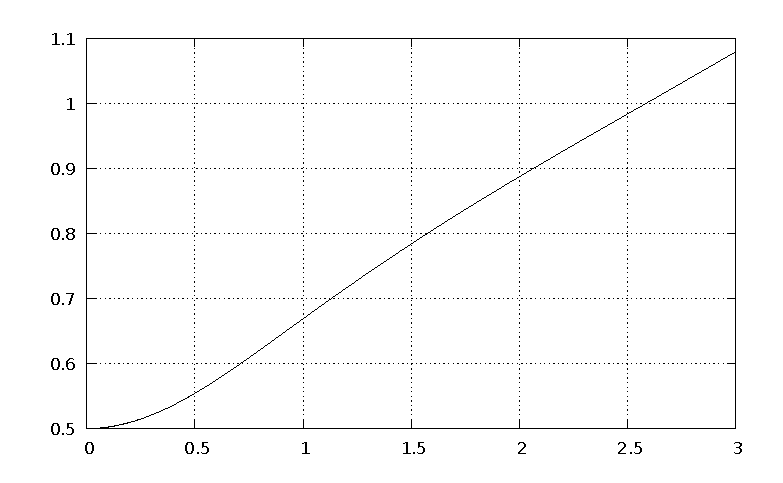
\includegraphics[width=.45\textwidth]
{figures/2d_benchmark1_barycenter_p0_nonlinear_128.ps}
\caption{Plot of the centre of mass over time for the simulation with 128
interface elements and using P2-P0 element and fixed point discretization.}
\label{fig:2d_benchmark1_barycenter}
\end{figure}

\begin{figure}[htbp]
\centering
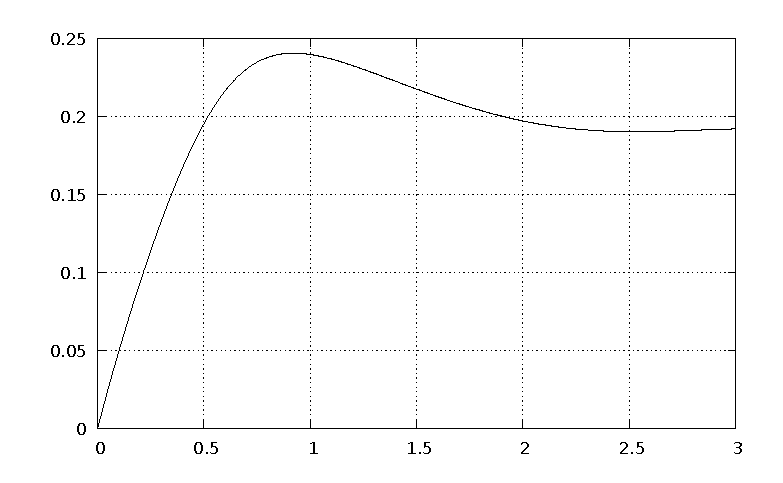
\includegraphics[width=.45\textwidth]
{figures/2d_benchmark1_velocity_p0_nonlinear_128.ps}
\caption{Plot of the average rising velocity over time for the simulation
with 128 interface elements and using P2-P0 element and fixed point
discretization.}
\label{fig:2d_benchmark1_velocity}
\end{figure}

\begin{figure}[htbp]
\centering
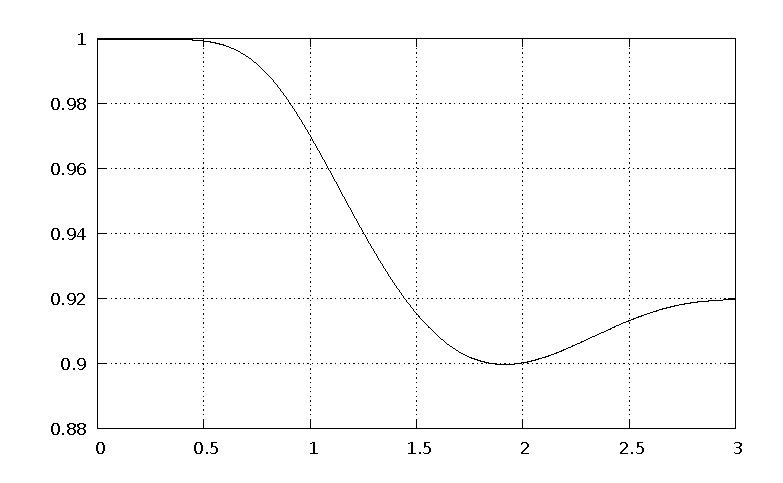
\includegraphics[width=.45\textwidth]
{figures/2d_benchmark1_circularity_p0_nonlinear_128.ps}
\caption{Plot of the circularity over time for the simulation with 128
interface elements and using P2-P0 element and fixed point discretization.}
\label{fig:2d_benchmark1_circularity}
\end{figure}

\begin{figure}[htbp]
\centering
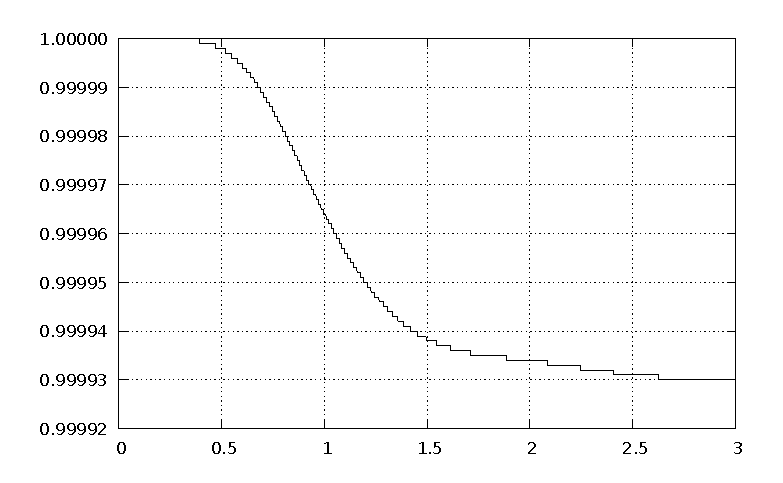
\includegraphics[width=.45\textwidth]
{figures/2d_benchmark1_inner_volume_p0_128.ps}
\caption{Plot of the relative inner volume
$\frac{\mathcal{L}^2(\Omega^m_-)}{\mathcal{L}^2(\Omega^0_-)}$ over time for the
simulation with 128 interface elements and using P2-P0 element and fixed point
discretization.}
\label{fig:2d_benchmark1_volume}
\end{figure}

\setcounter{equation} 0
\subsection{True solution benchmark}

Let $\Gamma(t) = \{ \vec z \in \R^d : |\vec z| = r(t)\}$ be a sphere of radius
$r(t)$ and curvature $\kappa(t) = -\,\frac{d-1}{r(t)}$.
An exact solution to the problem
(\ref{eq:full_momentum})-(\ref{eq:full_initial_interface}) with
(\ref{eq:full_velocity}) substitute by $\nabla\,.\,\vec u = \alpha\,d$ is
\begin{equation} \label{eq:r_benchmark1}
r(t) = \mathrm{e}^{\alpha\,t}\,r(0)\,,
\end{equation}
together with
\begin{equation} \label{eq:up_benchmark1}
\vec u(\vec z, t) = \alpha\,\vec z \,, \quad
p(\vec z, t) = -\,\bigg(\gamma - 2\,\alpha\,\frac{\mu_+ - \mu_-}
{d-1}r(t)\bigg)\,\kappa(t)\,\left[ \charfcn{\Omega_-(t)} -
\frac{\mathcal{L}^d(\Omega_-(t))}{\mathcal{L}^d(\Omega)}\right],
\end{equation}
and with $\vec f(\vec z, t) = \rho\,\alpha^2\,\vec z$, where $\alpha \in \R$.

Another exact solution to the problem
(\ref{eq:full_momentum})-(\ref{eq:full_initial_interface}) with
(\ref{eq:full_velocity}) substitute by $\nabla\,.\,\vec u = \big( \alpha_1 +
\alpha_2\charfcn{\Omega_+(t)}\big(\frac{2+d}{d}|\vec z|^2-r(t)^2\big)\big)d$ is
\begin{equation} \label{eq:r_benchmark2}
r(t) = \mathrm{e}^{\alpha_1\,t}\,r(0)\,,
\end{equation}
together with
\begin{align} \label{eq:up_benchmark2}
& \vec u(\vec z, t) = \bigg(\alpha_1+\alpha_2\charfcn{\Omega_+(t)}(|\vec
z|^2-r(t)^2)\bigg)\,\vec z\,, \\
& p(\vec z, t) = -\,\bigg(\gamma - 4\,\alpha_2\,\frac{\mu_+}{d-1}r(t)^3
\bigg)\,\kappa(t)\,\left[ \charfcn{\Omega_-(t)} -
\frac{\mathcal{L}^d(\Omega_-(t))}{\mathcal{L}^d(\Omega)}\right],
\end{align}
and with
\begin{align}
\vec f(\vec z, t) = &
\rho\,\bigg(\alpha_1^2\,+\charfcn{\Omega_+(t)}\bigg(-2\alpha_1\alpha_2r(t)^2 +
2\alpha_1\alpha_2\big(2|\vec z|^2-r(t)^2\big)+ \nonumber \\
& \alpha_2^2\big(|\vec z|^2-r(t)^2\big)\big(3|\vec z|^2 -
r(t)^2\big)-4(d+1)\alpha_2\frac{\mu_+}{\rho}\bigg)\bigg)\vec z
\end{align}
where $\alpha_1,\alpha_2 \in \R$.

Finally, a nontrivial divergence free and radially symmetric
solution $\vec u$ can be constructed on a domain that does not contain the
origin. To this end, consider e.g.\ $\Omega = (-1,1)^d \setminus [-\frac13,
\frac13]^d$, and let $\alpha \geq 0$ be given. Then, the expanding sphere where
\begin{equation} \label{eq:r_benchmark3}
r(t) = ([r(0)]^d + \alpha\,t\,d)^\frac1d \,,
\end{equation}
together with
\begin{equation} \label{eq:up_benchmark3}
\vec u(\vec z, t) = \alpha\,\frac{\vec z}{|\vec z\,|^d}\,, \quad
p(\vec z, t) = -\,\bigg(\gamma +2\,\alpha\,\frac{\mu_+ - \mu_-}
{r(t)^{d-1}}\bigg)\,\kappa(t)\,\left[ \charfcn{\Omega_-(t)} -
\frac{\mathcal{L}^d(\Omega_-(t))}{\mathcal{L}^d(\Omega)}\right],
\end{equation}
and with
\begin{equation}
\vec f(\vec z, t) = (1-d)\alpha^2\frac{\vec z}{|\vec z|^{2d}}
\end{equation}
is an exact solution to the problem
(\ref{eq:full_momentum})-(\ref{eq:full_initial_interface}) with
(\ref{eq:full_velocity}) substitute by $\nabla\,.\,\vec u =) = \alpha\,|\vec
z|^{-d}\,\vec z$.

In the following, unless otherwise stated, we choose the initial surface
$\Gamma(0) = \{ \vec z \in \R^d : |\vec z| = \frac12 \}$, the domain
$\Omega = (-1,1)^d$ and we employ uniform time steps $\tau_m=\tau$,
$m=0,\ldots, M-1$.

\bibliographystyle{siam}
\bibliography{../../bib/robert_refs,../../bib/marco_refs}
\end{document}
